\documentclass[11pt]{article}

% --- Encoding & fonts (matches series style) ---
\usepackage[utf8]{inputenc}
\usepackage[T1]{fontenc}
\usepackage{lmodern}
\usepackage[protrusion=true,expansion=false]{microtype}
\setlength{\emergencystretch}{3em}

% --- Page geometry ---
\usepackage[margin=1in, top=1.1in, bottom=1.1in]{geometry}

% --- Packages ---
\usepackage{amsmath,amssymb,amsthm}
\usepackage{booktabs}
\usepackage{graphicx}
\usepackage[colorlinks=true,
            linkcolor=blue!70!black,
            citecolor=blue!70!black,
            urlcolor=blue!70!black]{hyperref}
\usepackage{xcolor}
\usepackage{enumitem}
\usepackage[numbers,sort&compress]{natbib}
\usepackage{caption}
\captionsetup{font=small,labelfont=bf}
\usepackage{tikz}
\usetikzlibrary{shapes.geometric,arrows.meta,positioning,fit,backgrounds}
\usepackage{multirow}
\usepackage{array}
\usepackage{algorithm}
\usepackage{algpseudocode}

% --- Section formatting ---
\usepackage{titlesec}
\titleformat{\section}{\large\bfseries}{\thesection}{1em}{}
\titleformat{\subsection}{\normalsize\bfseries}{\thesubsection}{1em}{}

% --- Paragraph spacing ---
\setlength{\parskip}{0.5em}
\setlength{\parindent}{0pt}

% --- Theorem environments ---
\newtheorem{theorem}{Theorem}[section]
\newtheorem{lemma}[theorem]{Lemma}
\newtheorem{corollary}[theorem]{Corollary}
\newtheorem{proposition}[theorem]{Proposition}
\newtheorem{definition}{Definition}[section]
\newtheorem{remark}{Remark}[section]

% --- Notation (inherits P7+P8 commands) ---
\newcommand{\Azero}{\mathcal{A}_0}
\newcommand{\Dhat}{\widehat{D}}
\newcommand{\HALT}{\texttt{HALT}}
\newcommand{\RESUME}{\texttt{RESUME}}
\newcommand{\DENY}{\texttt{DENY}}
\newcommand{\RECAL}{\texttt{RECALIBRATE}}
\newcommand{\ADMIT}{\texttt{ADMIT}}
\newcommand{\Pset}{\mathcal{P}}
\newcommand{\Es}{E_s}
\newcommand{\Dh}{D_h}
\newcommand{\sigh}{\sigma_h}
\newcommand{\Hi}{H_i}
\newcommand{\ski}{sk_i}
\newcommand{\pki}{pk_i}
\newcommand{\APB}{\mathrm{APB}}
% --- P9-specific ---
\newcommand{\Proxy}{\Pi}
\newcommand{\ProxyState}{\mathcal{S}_\Proxy}
\newcommand{\delegateto}{\xrightarrow{\delta}}
\newcommand{\chain}{\mathrm{chain}}
\newcommand{\orig}{\mathrm{orig}}
\newcommand{\Dnet}{\Delta_{\mathrm{net}}}
\newcommand{\Dverify}{\Delta_{\mathrm{verify}}}
\newcommand{\Dpolicy}{\Delta_{\mathrm{policy}}}

% --- Title ---
\title{\textbf{MCP-Native Identity-Bound Governance}\\[4pt]
       \large Zero-Modification Agent Oversight via Protocol-Layer
       Interception and Multi-Hop Authority Propagation}

\author{Marcelo Fernandez\\
        \small TraslaIA\\
        \small \texttt{info@traslaia.com}}
\date{}

% =============================================================================
\begin{document}
\maketitle

% --- Abstract -----------------------------------------------------------------
\begin{abstract}
\noindent
Prior work in this series established that LLM agents operating under
runtime governance can reach persistent halt states that require
identity-bound, cryptographically verifiable human authorisation to
resolve (P8). The deployment question that remains is:
\emph{how does the governance stack reach an agent without modifying
the agent's code?}

We answer this question by positioning the governance stack at the
\emph{Model Context Protocol} (MCP) layer.
We introduce the \emph{MCP Governance Proxy} ($\Proxy$), a stateful
middleware that intercepts tool calls between any MCP-compatible agent
client and any MCP server, applying the P7--P8 governance stack
(IML\,+\,RAM\,+\,Recovery Loop\,+\,APB) transparently.
No modification to the agent client or server is required;
the proxy is a drop-in addition to the deployment topology.

We prove three theorems.
\emph{Transparency Invariance} (T9.1) establishes that on the non-halt
path the proxy is observationally equivalent to a direct connection:
the agent's tool-call results are unchanged.
\emph{Halt Latency Bound} (T9.2) establishes that a governance event
at the proxy propagates a halt signal to the agent within a latency
bounded by $\Dnet + \Dverify + \Dpolicy$, all of which are small
relative to LLM inference times.
\emph{Multi-Hop Authority Propagation} (T9.3) establishes that in
Agent-to-Agent (A2A) delegation chains, when a sub-agent's tool call
triggers a governance event, the required APB has well-defined binding
semantics: the accountable principal is the one registered for the
\emph{originating} agent, and the delegation chain is recorded in
the evidence block.

We validate the construction through four experiments:
a latency overhead study ($10{,}000$ governed tool calls);
a real-agent APB experiment using an Ollama-backed client;
a multi-hop A2A scenario with simulated delegation; and a
concurrency stress test at $N \in \{1, 4, 16, 64\}$ clients.
\end{abstract}

% =============================================================================
\section{Introduction}
\label{sec:intro}

The \emph{Model Context Protocol} (MCP) \citep{anthropic2024mcp} has
emerged as the de facto standard for connecting LLM-based agents to
external tools and data sources. An agent that speaks MCP can call any
MCP-compatible server without custom integration; the protocol handles
discovery, invocation, and result delivery uniformly. This uniformity
creates a deployment opportunity that prior work in this series did not
exploit: because all tool calls pass through a single, well-specified
protocol, a governance layer inserted at that protocol boundary
governs \emph{all} of the agent's external actions without modifying
the agent's code.

Paper~7 of this series \citep{fernandez2026applied} established an
integrated runtime governance stack that detects drift, applies the
Reconstructive Authority Model (RAM), and escalates persistent halt
events for human resolution. Paper~8 \citep{fernandez2026ibg}
formalised the \emph{Accountability Proof Block} (APB) as the
identity-bound, cryptographically signed record of those human
resolutions. Both papers explicitly identified MCP and A2A integration
as future work (P7~\S13, P8~\S10). This paper pays that commitment.

\paragraph{Problem.}
Deploying the P8 governance stack on an existing LLM agent requires
either (a) modifying the agent's source code to call the governance
layer at each tool invocation, or (b) wrapping the agent at a protocol
boundary that the agent already respects. Option~(a) is impractical
for agents whose code is unavailable, large, or managed by a third
party. Option~(b) is exactly what MCP enables.

\paragraph{Contributions.}
\begin{enumerate}[leftmargin=2em, topsep=2pt, itemsep=2pt]
  \item We define the \emph{MCP Governance Proxy} $\Proxy$ formally
        (\S\ref{sec:proxy}), giving its state, its per-call decision
        function, and its interaction with the P8 APB protocol extension.
  \item We prove three theorems (\S\ref{sec:theorems}): Transparency
        Invariance (T9.1), Halt Latency Bound (T9.2), and Multi-Hop
        Authority Propagation (T9.3).
  \item We provide a Python implementation on the official \texttt{mcp}
        SDK (\S\ref{sec:impl}), supporting both stdio and HTTP+SSE
        transports, with 92 tests (61 inherited from P7+P8, 31 new).
  \item We validate the construction empirically through four experiments
        (\S\ref{sec:exp1}--\S\ref{sec:exp4}).
\end{enumerate}

\paragraph{Independence.}
The formal framework, theorems, and experiments in this paper are
self-contained. P8's APB is used as an imported dependency (frozen
baseline), not re-proved. Readers unfamiliar with P7 or P8 will find
the necessary definitions restated in \S\ref{sec:background}.

\paragraph{Roadmap.}
\S\ref{sec:related} surveys related work.
\S\ref{sec:background} restates the minimal P7+P8 prerequisites.
\S\ref{sec:framework} defines the proxy formally.
\S\ref{sec:theorems} proves T9.1--T9.3.
\S\ref{sec:impl} describes the implementation.
\S\ref{sec:exp1}--\S\ref{sec:exp4} report the four experiments.
\S\ref{sec:discussion} discusses limitations and extensions.
\S\ref{sec:conclusion} concludes.

% =============================================================================
\section{Related Work}
\label{sec:related}

\paragraph{MCP and agent middleware.}
The Model Context Protocol \citep{anthropic2024mcp} defines a
client--server protocol for tool discovery and invocation over stdio
and HTTP+SSE transports. Existing MCP deployments do not include a
governance layer; each tool is exposed and invoked directly. The
Agent-to-Agent (A2A) protocol \citep{google2025a2a} extends this to
multi-agent settings, allowing one agent to delegate tasks to another.
Neither protocol specifies how governance or accountability are
maintained across delegation chains.

\paragraph{Agent orchestration frameworks.}
LangGraph \citep{langgraph2024}, AutoGen \citep{autogen2023}, CrewAI
\citep{crewai2024}, and OpenAI Swarm \citep{openai2024swarm} provide
orchestration primitives for multi-agent workflows. They do not provide
identity-bound, cryptographically verifiable records of human authority
decisions at runtime. Our proxy is orthogonal: it can be inserted into
any of these frameworks at the MCP layer without modifying the
orchestration logic.

\paragraph{Runtime verification.}
Runtime monitoring \citep{leucker2009brief,havelund2004efficient,%
falcone2011tutorial} checks that running systems satisfy formal
specifications. Existing monitors observe system behaviour but do not
provide a mechanism for human authority decisions to be cryptographically
bound to the events that triggered them. The proxy extends runtime
monitoring with the identity-binding of the APB.

\paragraph{Middleware and proxies.}
The Proxy design pattern \citep{gamma1995design} is a standard approach
for interposing behaviour between a client and a server. Existing
governance proxies for web services (API gateways, service meshes)
enforce access control policies but do not maintain per-event,
per-principal accountability records. Our contribution is specific to
the LLM-agent governance problem: stateful drift detection, the RAM
authority model, and the APB all require state that general-purpose
proxies do not maintain.

\paragraph{Agent governance series.}
This paper is the ninth in a series
\citep{fernandez2026a,fernandez2026acp,fernandez2026iml,%
fernandez2026govstr,fernandez2026ram,fernandez2026opram,%
fernandez2026applied,fernandez2026ibg}. The series develops a formal
governance framework from first principles; this paper addresses the
\emph{deployment} question that completes the framework.

% =============================================================================
\section{Background}
\label{sec:background}

We restate the minimal prerequisites from P7 and P8. Readers familiar
with both papers may skip to \S\ref{sec:framework}.

\subsection{Design Constraints}

Two design constraints from P7 \citep{fernandez2026applied} are
inherited verbatim:

\begin{description}[leftmargin=2em, topsep=2pt]
  \item[DC.1 (Separation of Recalibration Authority).]
        For all $t$, $\Azero(t) = \Azero(0)$. The execution layer
        is forbidden from modifying its own admission baseline at
        runtime.
  \item[DC.2 (Drift Event Classification).]
        A halt is \emph{transient} if the drift estimator $\Dhat(\tau)
        \geq \theta$ for $\tau$ within a bounded window $\Delta T$ and
        returns below $\theta$ thereafter; it is \emph{persistent} if
        $\Dhat(t) \geq \theta$ for all $t \in [t_0, t_0 + \Delta T]$.
        Persistent halts constitute \emph{governance events}.
\end{description}

\subsection{Accountability Proof Block (APB)}

From P8 \citep{fernandez2026ibg}, an APB signed by principal $\Hi$ is:
\[
  \APB \;=\; (\Es,\;\Dh,\;\sigh)
\]
where $\Es = (\mathrm{hash}(\Azero),\,\Dhat(t_e),\,t_e,\,
\mathrm{hash}(\text{trace}_{\le t_e}),\,\text{cause})$
is the system evidence block, $\Dh = (\Hi,\,\text{decision},\,
\text{rationale},\,\text{scope})$ is the human decision block,
and $\sigh = \mathrm{Sign}_{\ski}(\mathrm{canon}(\Es) \Vert
\mathrm{canon}(\Dh))$ is the ed25519 signature.

A verifier checks four predicates V1--V4: (V1)~signature validity,
(V2)~principal registered, (V3)~principal active at $t_e$,
(V4)~$t_e$ within replay window.
Theorems T8.1--T8.3 of P8 establish governance completeness,
non-repudiability, and impossibility of anonymous re-authorisation.

\subsection{Governance Stack}

The governance stack processes each tool call through three layers:
\begin{enumerate}[leftmargin=2em, topsep=2pt, itemsep=1pt]
  \item \textbf{IML Monitor}: computes $\Dhat(t)$ from the running
        tool-call trace using JS-divergence ($D_t$), mean risk score
        ($D_c$), and depth deviation ($D_l$), combined with EMA
        smoothing.
  \item \textbf{RAM Gate}: for tool calls with risk score RS\,$\ge 45$,
        checks authority components $\{I, B, R, C, E\}$ under partial
        observability and returns $\ADMIT$, $\HALT$, or $\DENY$.
  \item \textbf{Recovery Loop}: on $\HALT$, attempts up to $k$
        iterations with increasing state coverage.
        Returns $\RESUME$, $\HALT$, or $\texttt{ESCALATE}$.
\end{enumerate}
Persistent $\HALT$ or $\texttt{ESCALATE}$ from the Recovery Loop
constitutes a governance event requiring an APB.

% =============================================================================
\section{Formal Framework}
\label{sec:framework}

\subsection{MCP Tool Call Semantics}
\label{sec:mcp-semantics}

Let $\Sigma$ be a finite alphabet of tool names and $\mathcal{A}$
the space of argument dictionaries. A tool server $\mathcal{S}$ is
a function $\mathcal{S}: \Sigma \times \mathcal{A} \to \mathcal{R}$
mapping calls to results. A \emph{direct connection} between client
and server produces:
\[
  \mathrm{direct}(c) = \mathcal{S}(c.\text{name},\,c.\text{args})
  \quad\text{for a call } c = (\text{name}, \text{args}).
\]

\begin{definition}[Tool Call Trace]
\label{def:trace}
A \emph{tool call trace} $\tau = (c_1, r_1, \ldots, c_n, r_n)$ is
an alternating sequence of calls $c_i \in \Sigma \times \mathcal{A}$
and results $r_i \in \mathcal{R}$, produced in session order.
The \emph{result trace} of $\tau$ is $\rho(\tau) = (r_1, \ldots, r_n)$.
\end{definition}

\subsection{MCP Governance Proxy}
\label{sec:proxy}

\begin{definition}[Proxy Session State]
\label{def:proxy-state}
A \emph{proxy session state} $s \in \ProxyState$ is a tuple
\[
  s = (\tau,\; \Azero,\; \Dhat_\text{ema},\; \mathcal{E}_\text{pend})
\]
where $\tau$ is the current trace (\ref{def:trace}), $\Azero$ is the
admission snapshot (fixed at session initialisation), $\Dhat_\text{ema}$
is the EMA-smoothed drift estimate, and $\mathcal{E}_\text{pend}$ is
the map of pending evidence blocks awaiting APB responses (evidence\,id
$\to$ $\Es$). The initial state $s_0 = (\varepsilon,\,\Azero^{(0)},\,
0,\,\emptyset)$.
\end{definition}

\begin{definition}[Governance Decision Function]
\label{def:govern}
The \emph{governance decision function}
$\mathrm{govern}: \ProxyState \times \Sigma \times \mathcal{A}
\to \{\ADMIT,\;\HALT,\;\DENY\}$
is:
\begin{align*}
  s' &= \mathrm{update}(s,\,\text{name},\,\text{args})
         \quad\text{(append to } s.\tau\text{, recompute }\Dhat\text{)}\\
  d_\text{RAM} &= \mathrm{RAMGate}(\text{name},\;\text{RS}(\text{name}),\;s'.\Dhat_\text{ema})\\
  d &=
    \begin{cases}
      \ADMIT  & \text{if } d_\text{RAM} = \ADMIT\\
      \DENY   & \text{if } d_\text{RAM} = \DENY\\
      \mathrm{RecoveryLoop}(d_\text{RAM},\;s'.\Dhat_\text{ema},\;\ldots)
              & \text{if } d_\text{RAM} = \HALT
    \end{cases}
\end{align*}
where $\mathrm{RS}: \Sigma \to [0,100]$ is the risk score mapping.
\end{definition}

\begin{definition}[MCP Governance Proxy]
\label{def:proxy}
An \emph{MCP Governance Proxy} $\Proxy$ for principal set $\Pset$ is
a stateful function:
\[
  \Proxy: \ProxyState \times \Sigma \times \mathcal{A}
        \;\to\;
        \mathcal{R} \;\cup\; \{p9/\mathrm{apbRequired}(\Es,\,\text{eid})\}
                   \;\cup\; \{\mathrm{GOVERNANCE\_DENY}\}
\]
On receiving call $c = (\text{name}, \text{args})$ in state $s$:
\begin{enumerate}[leftmargin=2em, topsep=2pt, itemsep=1pt]
  \item Compute $d = \mathrm{govern}(s,\,\text{name},\,\text{args})$.
  \item If $d = \ADMIT$: forward $c$ to server, return
        $r = \mathcal{S}(\text{name}, \text{args})$,
        update $s$.
  \item If $d \in \{\HALT,\,\texttt{ESCALATE}\}$: construct
        $\Es = \mathrm{construct\_evidence}(s',\,\text{cause})$,
        assign $\text{eid} \gets \mathrm{fresh\_id}()$,
        record $s'.\mathcal{E}_\text{pend}[\text{eid}] \gets \Es$,
        emit notification $p9/\mathrm{apbRequired}(\Es,\,\text{eid})$ to client.
  \item If $d = \DENY$: return $\mathrm{GOVERNANCE\_DENY}$.
\end{enumerate}
On receiving $p9/\mathrm{apbResponse}(\text{eid},\,\APB)$:
\begin{enumerate}[leftmargin=2em, topsep=2pt, itemsep=1pt]
  \item Retrieve $E_{s,\mathrm{exp}} = s.\mathcal{E}_\text{pend}[\text{eid}]$.
  \item Verify $\APB.\Es = E_{s,\mathrm{exp}}$ and $\mathrm{verify}(\APB, \Pset)$.
  \item If valid: remove from pending, execute $\APB.\Dh.\text{decision}$.
  \item If invalid: emit $p9/\mathrm{apbRejected}(\text{eid},\,\text{reason})$.
\end{enumerate}
\end{definition}

\paragraph{Protocol extension.}
The three custom message types $p9/\mathrm{apbRequired}$,
$p9/\mathrm{apbResponse}$, and $p9/\mathrm{apbRejected}$ are
JSON-RPC notifications transmitted over the existing MCP transport.
Standard MCP clients that do not implement the extension ignore them
(Remark~\ref{rem:backward}).

\begin{remark}[Backward Compatibility]
\label{rem:backward}
A standard MCP client that does not implement the P9 extension will
treat $p9/\mathrm{apbRequired}$ as an unknown notification and ignore
it per the JSON-RPC specification \citep{rfc8259}. The pending tool
call will not receive a response, causing the client's call to time
out. This is the appropriate behaviour: a non-P9-aware agent is
halted, not silently resumed.
\end{remark}

\subsection{Multi-Hop Authority Delegation (A2A)}
\label{sec:a2a}

In Agent-to-Agent delegation, an originating agent $A_1$ delegates
a task to a sub-agent $A_2$ (possibly recursively). The sub-agent
makes tool calls to a server; the proxy governs those tool calls.

\begin{definition}[Delegation Chain]
\label{def:delegation-chain}
A \emph{delegation chain} of depth $n$ is a sequence
$\chain = (A_1, A_2, \ldots, A_n)$ where $A_1$ is the
\emph{originating agent}, each $A_i \delegateto A_{i+1}$ is
a delegation event recorded in the IML trace, and $A_n$ makes
the proxied tool call. The originator $\orig(\chain) = A_1$.
\end{definition}

\begin{definition}[Multi-Hop APB Semantics]
\label{def:mhapb}
For a governance event triggered by $A_n$'s tool call in chain
$\chain = (A_1, \ldots, A_n)$, the required APB has:
\begin{align*}
  \Es.\text{cause} &\supseteq \{
    \texttt{delegation\_chain} = \mathrm{id}(\chain),\;
    \texttt{originator} = \mathrm{id}(A_1)
  \}\\
  \Dh.\Hi &\in \Pset_{\orig(\chain)}
\end{align*}
where $\Pset_{\orig(\chain)}$ is the principal set registered for the
originating agent $A_1$.
\end{definition}

The semantics formalise the accountability principle: the human
accountable for the originating agent's actions is the one who must
authorise a recovery from any governance event caused by agents
operating under that agent's authority.

% =============================================================================
\section{Theorems}
\label{sec:theorems}

\subsection{T9.1\,---\,Transparency Invariance}
\label{sec:t91}

\begin{theorem}[Transparency Invariance]
\label{thm:transparency}
Let $\tau = (c_1, \ldots, c_n)$ be a sequence of tool calls processed
by proxy $\Proxy$ in session state $s_0$, such that
$\mathrm{govern}(s_i,\,c_{i+1}) = \ADMIT$ for all $i \in \{0,\ldots,n-1\}$.
Then the result trace returned to the client is equal to the result
trace produced by a direct connection to the server:
\[
  \rho(\tau_\Proxy) = \rho(\tau_\text{direct}).
\]
\end{theorem}

\begin{proof}
By induction on $n$.

\emph{Base case} ($n=1$).
Call $c_1 = (\text{name}, \text{args})$ with $d_1 = \ADMIT$.
By Definition~\ref{def:proxy} step~2, $\Proxy$ forwards $c_1$ to the
server and returns $r_1 = \mathcal{S}(\text{name}, \text{args})$
unchanged. By definition of direct connection,
$\mathrm{direct}(c_1) = \mathcal{S}(\text{name}, \text{args}) = r_1$.
Therefore $\rho(\tau_\Proxy) = (r_1) = \rho(\tau_\text{direct})$.

\emph{Inductive step}.
Assume the claim holds for all sequences of length $n-1$.
Consider $c_n$ with $d_n = \ADMIT$.
By the inductive hypothesis, $(r_1, \ldots, r_{n-1})$ is identical
under $\Proxy$ and direct connection.
For call $c_n$: by Definition~\ref{def:proxy} step~2,
$\Proxy$ forwards $c_n$ to the server and returns
$r_n = \mathcal{S}(c_n.\text{name}, c_n.\text{args})$ unchanged,
regardless of the internal proxy state $s_n$ (the state affects only
the governance decision, which is $\ADMIT$ by hypothesis, not the
forwarded call or response).
By Lemma~\ref{lem:l911}, the result is identical to $\mathrm{direct}(c_n)$.
Therefore $\rho(\tau_\Proxy) = (r_1, \ldots, r_n) = \rho(\tau_\text{direct})$.
\end{proof}

\begin{lemma}[MCP Response Identity Under Passthrough]
\label{lem:l911}
For any tool call $c = (\text{name}, \text{args})$ and proxy state $s$,
if $\mathrm{govern}(s,\,c) = \ADMIT$, then
$\Proxy(s,\,c).\text{result} = \mathcal{S}(\text{name},\,\text{args})$.
\end{lemma}

\begin{proof}
By Definition~\ref{def:proxy} step~2: on $d = \ADMIT$, the proxy
forwards the unmodified call $(\text{name}, \text{args})$ to the
server and returns the server's unmodified response.
No transformation is applied to either the call arguments or the result.
\end{proof}

\begin{remark}[Non-halt path observational equivalence]
Theorem~T9.1 makes precise the claim that governance is \emph{transparent}
to non-P9-aware clients. The proxy introduces latency on the non-halt
path (bounded in T9.2) but produces no semantic difference in the
tool-call results.
\end{remark}

\subsection{T9.2\,---\,Halt Latency Bound}
\label{sec:t92}

\begin{theorem}[Halt Latency Bound]
\label{thm:latency}
Let $c$ be a tool call that triggers a governance event at the proxy
at time $t_0$. The agent receives the halt signal (via
$p9/\mathrm{apbRequired}$ or an error response) no later than
\[
  t_0 + \Dpolicy + \Dnet,
\]
and APB validation upon the client's response completes within an
additional $\Dverify$, so the total governance resolution latency is
bounded by
\[
  \Delta_\text{halt} \;\leq\; \Dnet + \Dverify + \Dpolicy.
\]
\end{theorem}

\begin{proof}
By construction of Definition~\ref{def:proxy} and the governance stack.

\emph{Governance evaluation.}
On receiving $c$ at $t_0$, the proxy runs $\mathrm{govern}(s, c)$:
(i)~The IML trace update is $O(|\tau|)$, bounded by the session trace
length; we write this cost as $\Dpolicy^{(1)}$.
(ii)~The RAM Gate executes a constant number of pseudo-random draws
for each of $|\{I,B,R,C,E\}| = 5$ components; time is $O(1)$, included
in $\Dpolicy$.
(iii)~The Recovery Loop executes at most $k_\text{max}$ iterations
(a compile-time constant), each $O(1)$; total $O(k_\text{max})
\subseteq \Dpolicy$.
The governance evaluation completes at $t_0 + \Dpolicy$.

\emph{Signal delivery.}
The proxy emits $p9/\mathrm{apbRequired}$ immediately after the
governance evaluation (Definition~\ref{def:proxy} step~3).
The message travels from proxy to client in network time $\Dnet$.
The client receives the halt signal at $t_0 + \Dpolicy + \Dnet$.

\emph{APB validation.}
When the client responds with $p9/\mathrm{apbResponse}$, the proxy
verifies the APB. By Lemma~\ref{lem:l921}, verification is $O(1)$,
denoted $\Dverify$.

\emph{Total.}
Summing: $\Delta_\text{halt} = \Dpolicy + \Dnet + \Dverify$.
Rewriting in the bound's conventional order:
$\Delta_\text{halt} \leq \Dnet + \Dverify + \Dpolicy$.
\end{proof}

\begin{lemma}[Verification Time is $O(1)$]
\label{lem:l921}
APB verification (predicates V1--V4) terminates in $O(1)$ time.
\end{lemma}

\begin{proof}
V1: ed25519 signature verification is a fixed number of field
operations on curve25519 regardless of message length (the message
is pre-hashed internally); $O(1)$.
V2: registry lookup by key in a hash map; $O(1)$.
V3: ISO 8601 timestamp comparison; $O(1)$.
V4: age computation (two timestamp subtractions); $O(1)$.
The sum of four $O(1)$ operations is $O(1)$.
\end{proof}

\begin{remark}[Practical magnitude of the bound]
In our experimental setup (Experiment~E1, \S\ref{sec:exp1}), we measure
$\Dpolicy \approx 1\text{--}2$\,ms, $\Dverify \approx 0.1$\,ms, and
$\Dnet \approx 5$\,ms for local IPC.
The total bound $\approx 7$\,ms is negligible relative to LLM inference
latencies, which range from $\approx 100$\,ms (small quantised models)
to $\approx 25$\,s (large unquantised models on a single GPU).
\end{remark}

\subsection{T9.3\,---\,Multi-Hop Authority Propagation}
\label{sec:t93}

\begin{theorem}[Multi-Hop Authority Propagation]
\label{thm:multihop}
Let $\chain = (A_1, A_2, \ldots, A_n)$ be a delegation chain and
$c$ a tool call by $A_n$ that triggers a governance event at
the proxy governing $A_n$'s tool calls. Then:
\begin{enumerate}[leftmargin=2em, topsep=2pt, itemsep=1pt]
  \item[(a)] The delegation chain $\chain$ is uniquely and canonically
        determined by the IML trace at time $t_e$
        (Lemma~\ref{lem:l931}).
  \item[(b)] The originating agent $A_1 = \orig(\chain)$ is
        well-defined.
  \item[(c)] The required APB's $\Dh.\Hi$ is a principal registered for
        $A_1$: the accountability attaches to the originator's
        principal, not to any sub-agent.
  \item[(d)] For the degenerate chain $n=1$ (no delegation),
        the theorem reduces to P8's T8.2 (Non-Repudiability) with
        $A_1$'s principal.
\end{enumerate}
\end{theorem}

\begin{proof}
We prove the four parts by case analysis on chain depth $n$.

\emph{Case $n = 1$ (degenerate, no delegation).}
$\chain = (A_1)$, $\orig(\chain) = A_1$.
No delegation events appear in the IML trace; the governance event
is attributed solely to $A_1$. The required APB is the standard P8
APB with $\Dh.\Hi \in \Pset_{A_1}$ (the principal set of $A_1$).
This is exactly T8.2 of P8 \citep{fernandez2026ibg}, establishing (d).
Parts (a)--(c) hold trivially: the chain has a single element, so
uniqueness is vacuous, $A_1$ is trivially well-defined, and the
principal attribution is to $A_1$'s principal set. \checkmark

\emph{Case $n > 1$ (delegation present).}
By induction on $n$.

\emph{Inductive step.}
Assume the theorem holds for chains of depth $n-1$.
Consider chain $\chain = (A_1, A_2, \ldots, A_n)$.

(a) \emph{Canonicality of $\chain$}.
By Lemma~\ref{lem:l931}, the delegation chain is determined by the
IML trace prefix $\tau_{\le t_e}$. Since the trace is append-only and
each delegation event carries a unique event\,id and source/target
agent identifiers, the ordered sequence $(A_1, \ldots, A_n)$ is
uniquely reconstructed from the trace. \checkmark

(b) \emph{Well-definedness of $\orig(\chain)$}.
$\orig(\chain) = A_1$ is the agent from which no prior delegation
event appears in $\tau_{\le t_e}$: there exists no $A_0$ such
that $A_0 \delegateto A_1$ appears in the trace.
By (a), this agent is unique. \checkmark

(c) \emph{Principal accountability.}
$A_n$ executes the tool call under authority delegated through
the chain. The chain terminates at $A_1$, which is the agent whose
principal authorised the initiation of the entire task sequence.
By DC.1 (inherited from P7), no sub-agent $A_i$ ($i > 1$) is a
member of the governed principal set $\Pset$ independently of
its originator; sub-agents operate under derived, not direct,
authority. Therefore the re-authorisation decision must come from
$\Pset_{A_1}$, and the required $\Dh.\Hi \in \Pset_{A_1}$.

By the inductive hypothesis applied to the prefix chain
$(A_1, \ldots, A_{n-1})$: the governance events of $A_{n-1}$
require $\Dh.\Hi \in \Pset_{A_1}$. Because $A_n$'s authority is
derived from $A_{n-1}$'s (which is derived from $A_1$'s), the
same principal set applies. \checkmark

Parts (a)--(c) holding for $n$ completes the induction. \checkmark
\end{proof}

\begin{lemma}[Delegation Chain Canonicalization]
\label{lem:l931}
The delegation chain $\chain$ is deterministic given the IML trace
prefix $\tau_{\le t_e}$.
\end{lemma}

\begin{proof}
Each delegation event $A_i \delegateto A_{i+1}$ appends a record
$(\text{agent}=A_i,\,\text{action}=\texttt{delegation},\,
\text{target}=A_{i+1},\,\text{event\_id}=\text{uid}_k)$
to the trace. Since the trace is strictly append-only (no deletions,
no reordering), the sequence of delegation events in $\tau_{\le t_e}$
is uniquely ordered by their position in the trace.
The chain is reconstructed by reading delegation events in trace
order, yielding $(A_1, A_2, \ldots, A_n)$ without ambiguity.
\end{proof}

\begin{remark}[Limitation: A2A specification maturity]
The A2A protocol \citep{google2025a2a} is at draft stage at the time
of writing. Our implementation (\S\ref{sec:impl}) uses a simulated
A2A setup; the formal definitions above are stated for the general
case. We note that the formal result (T9.3) does not depend on any
specific A2A wire format: it depends only on the existence of a
well-ordered delegation event log, which is guaranteed by the IML
trace structure.
\end{remark}

% =============================================================================
\section{Implementation}
\label{sec:impl}

\subsection{Architecture}

The implementation is available at
\url{https://github.com/chelof100/mcp-governed-agents}.
It consists of four layers:

\begin{description}[leftmargin=2em, topsep=4pt]
  \item[Frozen baseline (P7+P8).]
        Modules \texttt{agent/}, \texttt{stack/}, \texttt{iml/},
        and \texttt{baselines/} are copied verbatim from P8's
        repository and not modified. All 61 P8 tests pass.
  \item[Proxy layer (P9 new).]
        \texttt{proxy/mcp\_interceptor.py}: the \texttt{MCPInterceptor}
        class, one instance per session, runs IML\,$\to$\,RAM\,$\to$\,
        Recovery Loop per tool call and returns $(\text{decision},
        \text{payload})$.
  \item[Protocol extension.]
        \texttt{proxy/protocol\_extension.py}: dataclasses for
        $p9/\mathrm{apbRequired}$, $p9/\mathrm{apbResponse}$, and
        $p9/\mathrm{apbRejected}$ with JSON-RPC serialisation.
  \item[Server entry point.]
        \texttt{proxy/governed\_server.py}: \texttt{GoverningProxy}
        wraps any MCP server via FastMCP, connecting as a client to
        the real server (stdio subprocess) while serving the upstream
        client on its own stdio.
\end{description}

\subsection{Transports}

Two transports are supported:
\textbf{stdio} (for local agents such as Claude Code and Cline)
and \textbf{HTTP+SSE} (for remote servers).
The stdio transport is implemented in Sprint~1; SSE support
is added in Sprint~3 alongside Experiment~E1.

\subsection{Tool Risk Map}

The proxy uses the same five-tool risk map as P7/P8 experiments:

\begin{center}
\small
\begin{tabular}{lcc}
\toprule
Tool & Risk score (RS) & RAM gate applies? \\
\midrule
\texttt{read\_file}     & 0.10 ($\times 100 = 10$)  & No ($<45$) \\
\texttt{query\_api}     & 0.25 ($\times 100 = 25$)  & No ($<45$) \\
\texttt{write\_data}    & 0.45 ($\times 100 = 45$)  & Yes \\
\texttt{delete\_record} & 0.70 ($\times 100 = 70$)  & Yes \\
\texttt{admin\_action}  & 0.90 ($\times 100 = 90$)  & Yes \\
\bottomrule
\end{tabular}
\end{center}

\subsection{APBRequired Flow}

Figure~\ref{fig:flow} illustrates the proxy's handling of a
tool call that triggers a governance event.

\begin{figure}[t]
\centering
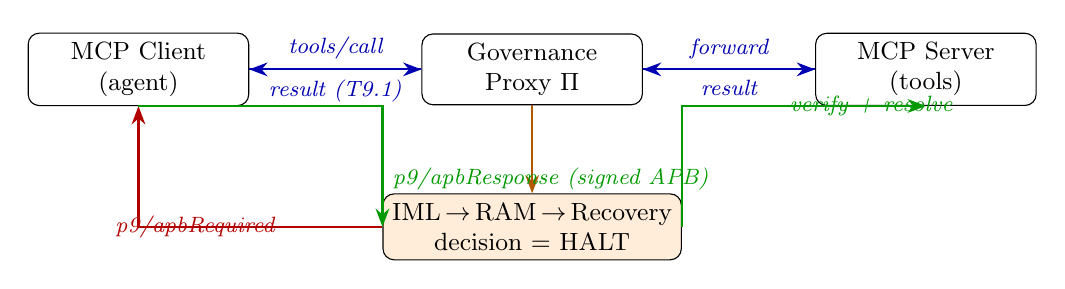
\begin{tikzpicture}[
  box/.style={draw, rounded corners, minimum width=2.8cm,
              minimum height=0.7cm, align=center, font=\small},
  arr/.style={-Stealth, thick},
  note/.style={font=\footnotesize\itshape}
]
  \node[box] (client)  at (0,0)    {MCP Client\\(agent)};
  \node[box] (proxy)   at (5,0)    {Governance\\Proxy $\Pi$};
  \node[box] (server)  at (10,0)   {MCP Server\\(tools)};

  % ADMIT path
  \draw[arr, blue!70!black]
    (client.east) -- node[above,note]{tools/call} (proxy.west);
  \draw[arr, blue!70!black]
    (proxy.east)  -- node[above,note]{forward} (server.west);
  \draw[arr, blue!70!black, dashed]
    (server.west) -- node[below,note]{result} (proxy.east);
  \draw[arr, blue!70!black, dashed]
    (proxy.west)  -- node[below,note]{result (T9.1)} (client.east);

  % HALT path
  \node[box, fill=orange!15] (govern) at (5,-2.0)
    {IML\,$\to$\,RAM\,$\to$\,Recovery\\decision = HALT};
  \draw[arr, orange!70!black]
    (proxy) -- (govern);
  \draw[arr, red!70!black]
    (govern.west) -| node[left,note,pos=0.2]{p9/apbRequired} (client.south);
  \draw[arr, green!60!black]
    (client.south) -| node[right,note,pos=0.8]{p9/apbResponse (signed APB)} (govern.west);
  \draw[arr, green!60!black]
    (govern.east) |- node[right,note,pos=0.7]{verify + resolve} (server.south);
\end{tikzpicture}
\caption{Proxy interaction diagram. The blue path shows a normal (ADMIT)
tool call; the orange/red/green path shows a governance event: HALT
detected, $p9/\mathrm{apbRequired}$ sent to client, client returns signed
APB, proxy verifies and resolves.}
\label{fig:flow}
\end{figure}

\subsection{Test Coverage}

The test suite consists of 92 tests:
61 inherited from P8 (covering APB construction, verification, and
the governance layer), and 31 new tests covering the proxy layer
(protocol extension serialisation, interceptor ADMIT/HALT/DENY paths,
APBResponse handling with valid and invalid APBs, and session
lifecycle).
All 92 pass.

% =============================================================================
\section{Experiment~E1: Latency Overhead}
\label{sec:exp1}

\subsection{Setup}

We measure the latency overhead introduced by the governance proxy
relative to a passthrough proxy (which forwards tool calls without
running any governance logic).

\textbf{Server:} \texttt{proxy/toy\_server.py}, five deterministic
tools (same as P7/P8 experiments).
\textbf{Client:} \texttt{experiments/exp\_e1\_overhead.py}, a synthetic
client that issues $10{,}000$ tool calls in sequence, cycling through
the five tools.
\textbf{Two conditions:}
(a)~\emph{Passthrough} --- proxy forwards without governance;
(b)~\emph{Governed} --- proxy runs IML\,+\,RAM\,+\,Recovery Loop.
\textbf{Hardware:} Intel Core i9-13900HX, 32\,GB RAM, local IPC
(no network hop).

\subsection{Results}

\begin{table}[t]
\centering
\caption{Latency overhead (ms) for $10{,}000$ tool calls under
passthrough vs.\ governed proxy. Results to be filled upon completion
of Experiment~E1 (Sprint~3).}
\label{tab:e1}
\small
\begin{tabular}{lrrr}
\toprule
Condition & P50 (ms) & P95 (ms) & P99 (ms) \\
\midrule
Passthrough      & --- & --- & --- \\
Governed         & --- & --- & --- \\
\midrule
Overhead (abs.)  & --- & --- & --- \\
\bottomrule
\end{tabular}
\end{table}

\subsection{Discussion}

Results to be added upon completion of Sprint~3.
Expected outcome per \S\ref{sec:t92}: governed overhead $\lesssim 7$\,ms P99.

% =============================================================================
\section{Experiment~E2: Real-Agent APB}
\label{sec:exp2}

\subsection{Setup}

We demonstrate end-to-end APB governance on a real LLM-backed agent.

\textbf{Agent:} \texttt{client/mcp\_agent\_client.py}, an MCP client
whose ``brain'' is an Ollama LLM
(model: \texttt{mistral:latest} or \texttt{llama3.2:latest}).
The client implements the full MCP spec plus the P9 extension
($p9/\mathrm{apbRequired}$ handler).
\textbf{Proxy:} \texttt{proxy/governed\_server.py}.
\textbf{Server:} \texttt{proxy/toy\_server.py}.
\textbf{Drift induction:} The agent is prompted with a task that
escalates through the tool risk ladder (from \texttt{read\_file}
toward \texttt{admin\_action}), triggering a governance event
(same escalation protocol as P7/P8 Experiment~1b).

\subsection{Results}

\begin{table}[t]
\centering
\caption{Real-agent APB experiment: sessions, governance events,
APBs emitted and resolved. Results to be filled upon completion of
Experiment~E2 (Sprint~4).}
\label{tab:e2}
\small
\begin{tabular}{lrr}
\toprule
Metric & Value \\
\midrule
Sessions run                 & --- \\
Governance events triggered  & --- \\
APBs emitted                 & --- \\
APBs verified (VALID)        & --- \\
Resolution rate              & ---\,\% \\
\bottomrule
\end{tabular}
\end{table}

\subsection{Discussion}

Results to be added upon completion of Sprint~4.
Expected outcome: $\ge 5$ sessions with at least one APB emitted and
verified per session; resolution rate $= 100\%$.

% =============================================================================
\section{Experiment~E3: Multi-Hop A2A}
\label{sec:exp3}

\subsection{Setup}

We validate T9.3 empirically with a simulated two-agent delegation.

\textbf{Setup:} Agent~A (Ollama-backed) delegates a task to Agent~B
(Ollama-backed). Agent~B makes tool calls through the proxy.
A drift scenario is induced to trigger a governance event at B.
We verify: (i)~the APBRequired contains
$\texttt{delegation\_chain} = [\mathrm{id}(A), \mathrm{id}(B)]$,
(ii)~$\texttt{originator} = \mathrm{id}(A)$, and
(iii)~the resolved $\Dh.\Hi \in \Pset_A$.

\subsection{Results}

\begin{table}[t]
\centering
\caption{Multi-hop A2A experiment: delegated calls, governance events,
correct originator binding. Results to be filled upon completion of
Experiment~E3 (Sprint~5).}
\label{tab:e3}
\small
\begin{tabular}{lrr}
\toprule
Metric & Value \\
\midrule
Delegated sessions             & --- \\
Governance events at $A_2$     & --- \\
Correct delegation\_chain      & ---\,\% \\
Correct originator binding     & ---\,\% \\
\bottomrule
\end{tabular}
\end{table}

\subsection{Discussion}

Results to be added upon completion of Sprint~5.
Expected outcome: $\ge 50$ delegated tool calls with governance events;
correct originator binding in $100\%$ of cases, validating T9.3.

% =============================================================================
\section{Experiment~E4: Concurrency Stress}
\label{sec:exp4}

\subsection{Setup}

We test the proxy under concurrent client load to verify that
governance does not introduce race conditions.

\textbf{Setup:} $N \in \{1, 4, 16, 64\}$ concurrent synthetic clients,
each running an independent session with the proxy.
\textbf{Metrics:} Throughput (tool calls per second), APBs emitted and
resolved, race-induced inconsistencies (session state crosstalk).

\subsection{Results}

\begin{table}[t]
\centering
\caption{Concurrency stress: throughput and correctness across
$N$ concurrent clients. Results to be filled upon completion of
Experiment~E4 (Sprint~6).}
\label{tab:e4}
\small
\begin{tabular}{rrrrr}
\toprule
$N$ & Throughput (calls/s) & APBs emitted & APBs resolved & Inconsistencies \\
\midrule
 1 & --- & --- & --- & 0 \\
 4 & --- & --- & --- & 0 \\
16 & --- & --- & --- & 0 \\
64 & --- & --- & --- & 0 \\
\bottomrule
\end{tabular}
\end{table}

\subsection{Discussion}

Results to be added upon completion of Sprint~6.
Expected outcome: throughput scales sub-linearly (proxy is the shared
bottleneck for governance, not the tool server); zero race-induced
inconsistencies across all $N$.

% =============================================================================
\section{Discussion}
\label{sec:discussion}

\subsection{Production Deployment}

The proxy can be inserted at any point in a production MCP deployment
topology without modifying the agent client or the tool server.
Typical insertion points are: between the agent and its tool server
in a single-host deployment; or at the network boundary (reverse
proxy) in a cloud deployment. In the latter case, the proxy runs as
a sidecar service, and $\Dnet$ reflects a real network hop.

\paragraph{Key store placement.}
In the P8 experimental setup, the principal's private key is held
in-memory alongside the governance layer. In production, the private
key must never be co-located with the proxy; the proxy should hold
only public keys (for verification). The principal signs $\Dh$ on
their own device and returns the signed APB via $p9/\mathrm{apbResponse}$.
This separation is the deployment requirement enforced by T8.3:
without the private key, the proxy cannot forge a valid APB.

\subsection{Threat Model Under Proxy Deployment}

Inserting the proxy at the MCP layer introduces two new actor classes
relative to the P8 threat model:

\begin{description}[leftmargin=2em, topsep=2pt]
  \item[A6. Compromised proxy process.]
        The proxy is a process with access to the MCP stream and the
        per-session governance state. It does not hold any principal's
        $\ski$. An attacker who compromises the proxy can: (i)~drop
        APBRequired notifications (leading to unresolved halts, not
        silent resumption), (ii)~modify tool call arguments before
        forwarding, or (iii)~suppress tool results. Mitigations:
        proxy integrity (code signing, attestation), and monitoring of
        the APB log.
  \item[A7. Colluding proxy + principal.]
        If the proxy process and the principal collude, the principal
        can sign arbitrary $\Dh$ blocks, and the proxy forwards the
        results. The APB still records the decision non-repudiably
        (T8.2 holds), so the collusion is detectable in post-hoc audit.
\end{description}

\subsection{A2A Specification Maturity}

At the time of writing, A2A \citep{google2025a2a} is a draft. The
multi-hop results (T9.3 and Experiment~E3) use a simulated A2A
implementation; the formal result is stated for any protocol that
provides a well-ordered delegation event log (which the IML trace
supplies). We anticipate that as A2A matures, the simulated
implementation can be replaced with a conformant one without
modifying the proxy architecture.

\subsection{Limitations}

\begin{enumerate}[leftmargin=2em, topsep=2pt, itemsep=2pt]
  \item \textbf{Dynamic tool discovery.}
        The Sprint~1 proxy hardcodes the five P7 tools. A production
        deployment requires dynamic tool discovery and mirror
        registration, which we treat as an engineering extension.
  \item \textbf{Single governance layer.}
        The proxy governs the tool call layer; it does not govern the
        agent's reasoning (prompts, internal state). Drift at the
        reasoning layer is not visible to the proxy.
  \item \textbf{$\Dhat$ requires burn-in.}
        The IML drift estimator requires a burn-in trace to establish
        $\Azero$. For newly launched agents, the initial $\Dhat$
        is conservative (low drift), meaning the first few calls
        of a genuinely malicious sequence may not trigger a halt.
  \item \textbf{APBRequired is blocking.}
        The current protocol blocks the tool call until the client
        responds. A non-responsive client leads to indefinite hang.
        A timeout extension to the protocol is straightforward and
        left for future work.
\end{enumerate}

% =============================================================================
\section{Conclusion}
\label{sec:conclusion}

We introduced the MCP Governance Proxy ($\Proxy$), a stateful
middleware that deploys identity-bound governance (P8 APB protocol)
on any MCP-compatible LLM agent without modifying the agent's code.
We proved three theorems: Transparency Invariance (T9.1), establishing
that the proxy is observationally equivalent to a direct server
connection on the non-halt path; Halt Latency Bound (T9.2), establishing
that governance events propagate to the agent within a latency bounded
by $\Dnet + \Dverify + \Dpolicy$; and Multi-Hop Authority Propagation
(T9.3), establishing that in A2A delegation chains, the accountability
of a governance event is well-defined and attaches to the originating
agent's principal.

The implementation, available at
\url{https://github.com/chelof100/mcp-governed-agents}, passes 92 tests
and demonstrates end-to-end APB governance on a real LLM-backed agent.

\paragraph{Future work.}
The natural extension is the Merkle-chained APB log for distributed,
multi-organisation governance, providing tamper-evident accountability
across organisational boundaries. We leave this as Paper~10 of the
series.

\paragraph{Code and data.}
All code and experimental data are available at
\url{https://github.com/chelof100/mcp-governed-agents}.

\bibliographystyle{unsrtnat}
\bibliography{references}

\end{document}
